\chapter{Computational details for chap. \ref{chap:pam-classical}}
\label{ap:a}
\label{ap:a-computational}

    In chapter \ref{chap:pam-classical} we built linear programs that can be used to certify classicality in the prepare and measure scenario. When $\eta$ --- the insphere radius (see fig. \ref{fig:measurements-hull}) --- approaches $1$, this method provides a necessary and sufficient condition for classicality. To make $\eta \rightarrow 1$, it is necessary to increase the number of probe measurements (or preparations). Decomposing the deterministic strategies $\lambda$ into their extremal points results in an exponentially large set, with $N_\lambda \propto B^{dY}$ extremal points. Even for reasonably sized instances, it becomes prohibitively expensive to even enumerate the strategies, let alone to solve the problem. Consequently, regardless of the efficiency of linear programming algorithms (sec. \ref{sec:linear-programming}), the size of our program instance that scales exponentially. This large amount of extremal strategies is the computational bottleneck of our approach. However, we can circumvent this issue using the approach we now describe (a similar procedure, for an analogous method applied to other correlation scenarios, is outlined in \cite{fillettaz_algorithmic_2018}).

	Our approach is to avoid working on --- and even enumerating --- all $N_\lambda$ extremal points at once. Instead, we iteratively explore the deterministic strategy space. To understand how, recall that the maximization programs discussed in chap. $\ref{chap:pam-classical}$ search for the optimal weights $\pi(\lambda)$ such that a convex combination of extremal points of the local polytope describe the behavior of our system. The optimization variable, $\alpha$, controls the amount of noise we have to put into the preparations (or measurements) so that a classical model exist. A solution will always exists, for the worst case $\alpha = 0$ corresponds to maximally mixed preparations (or measurements), which trivially have a classical model. As a result, any solved instance returns us the optimal value $\alpha$, and the weights $\pi(\lambda)$ used to attain it.

	A linear program searches for optimal solutions inside polyhedra. In our instances, the extremal points of the feasible region are the deterministic strategies themselves, and further constraints impose we are working on its convex hull. Carathéodory's Theorem \cite{rockafellar_convexanalysis_1970} states that at most $d+1$ extremal points are necessary to optimally describe any point of a $d$-dimensional convex set. This implies that, optimally, most of the $\pi(\lambda)$ found will be zero. We cannot know, beforehand, which points make for an optimal description, so we start by taking $N_\lambda^\prime \gg d+1$ --- but much smaller than $N_\lambda$ --- points, and optimizing over them. To set up the next iteration, we take the resulting $\pi(\lambda) = 0$  from this first step and replace them with previously unexplored deterministic strategies. Then we run the program with these as input. As, at each round, we are keeping all optimal $\lambda$ from the previous round, the optimal value $\alpha$ will be non-decreasing between iterations. Furthermore, for so large $Y$ that it would be prohibitive to enumerate and keep track of all previously visited strategies, we observe that simply randomly sampling $\lambda$'s on each run makes our procedure rapidly converge to an $\alpha^*$, which then assumes a constant value for all subsequent iterations. This result provides a lower bound on the maximum visibility imposed on the preparations such that their behavior is classical. Naturally, this procedure works for any of the linear programs we have constructed. More precisely, it goes like this

	%
	\IncMargin{1em}
	\begin{algorithm}[ht!]
	\setstretch{1.3}
		% Defs
		% \SetKwData{}
		\SetKwFunction{findmodel}{FindClassicalityModel}
		\SetKwFunction{sample}{SampleStrategies}
		\SetKwFunction{stop}{Stop?}
		\SetKwFunction{ccount}{Count}
		\SetKwFunction{append}{append}
		\SetKwFunction{remove}{remove}
		\SetKwFunction{length}{length}
		% Header
		\Input{$N_\lambda^\prime$, $\mathcal{S}$, $\mathcal{M}$, $\eta$, optional: $t$}
		\Output{$\alpha^*$}
		\BlankLine
		% Algo
		\nonl Let $\{ \alpha \}$ and $\{ \lambda \}$ be empty lists and $N_0 \longleftarrow N_\lambda^\prime$ \\
		\While{$\neg\stop(\{\alpha\})$}{
			$\{ \lambda \}.\append(\sample(d,B,X,Y,N_0))$ \\
			$\alpha^*, \pi(\lambda) \longleftarrow \findmodel(\mathcal{S}, \mathcal{M}, \eta, \{ \lambda \}, \text{optional: } t)$ \\
			$\{\alpha\}.\append(\alpha^*)$ \\
			$\{\lambda\}.\remove(\pi(\lambda) == 0)$ \\
			$N_0 \longleftarrow N_\lambda^\prime - \length(\{\alpha\})$ \\
		}
		\Return $\alpha^*$
		\vspace{.5em}
		%
		\caption{Iterating on the deterministic strategies space}
		\label{algo:iterative-strategy}
	\end{algorithm}
	\DecMargin{1em}
	%

	where \texttt{FindClassicalityModel} is one of programs \eqref{eq:measurement-classicality-projective}, \eqref{eq:preparation-classicality-povm}, \eqref{eq:measurement-classicality-projective} or \eqref{eq:preparation-classicality-povm}, the parameters $d, B, X, Y$ in \texttt{SampleStrategies} can be extracted from the inputs, and $\texttt{Stop?}$ implements some convergence criterion.

	To illustrate the procedure, consider the problem of certifying that the preparation set $\mathcal{S}(\theta, \phi) = \{ \rho_{\mathbf{x}}, \rho_{\mathbf{z}}, \rho_{\mathbf{r}(\theta, \phi)} \}$ is classical for projective measurements (i.e., \texttt{FindClassicalityModel} is program~\eqref{eq:preparation-classicality-projective}). Here, $\rho_{\mathbf{v}}$ denotes a qubit state with Bloch vector $\mathbf{v}$, and the unit vector $\mathbf{r}(\theta, \phi)$ is given by its spherical polar and azimuthal angles, respectively.

	Arranging our measurements operators as those associated to the vertices of an icosahedron ($Y = 6$ with $\eta \approx 0.79$), we get a fairly small problem that can be solved either directly or iteratively. Fig.~\ref{fig:hm-icos} shows the result through the iterative procedure, which exactly matches the direct approach. With twice the amount of measurements arranged as the vertices of a rhombicuboctahedron ($\eta \approx 0.86$), it is no longer possible to compute \ref{fig:hm-romb} in a direct manner. As a matter of fact, even enumerating all deterministic strategies turns costly. Employing the procedure here described allowed us to compute fig. \ref{fig:hm-romb}. The advantage of having more measurements then becomes evident, with the rhombicuboctahedron resulting in increased visibilities. We pay for that with more computation time: while the model for each preparation set in fig. \ref{fig:hm-icos} takes less than a minute to compute in a standard desktop computer, it takes around $7$ minutes for fig. \ref{fig:hm-romb} when using fairly robust parameters (likewise for figs. \ref{fig:hm-romb}, \ref{fig:nonclassicality-activation} and \ref{fig:incompatibility-vs-classicality}). Implementations for these and all forthcoming applications can be found at a public repository \cite{classicality_repository}.

	\begin{figure*}[t!]
        \centering
        \subfigure[Icosahedron]{\label{fig:hm-icos}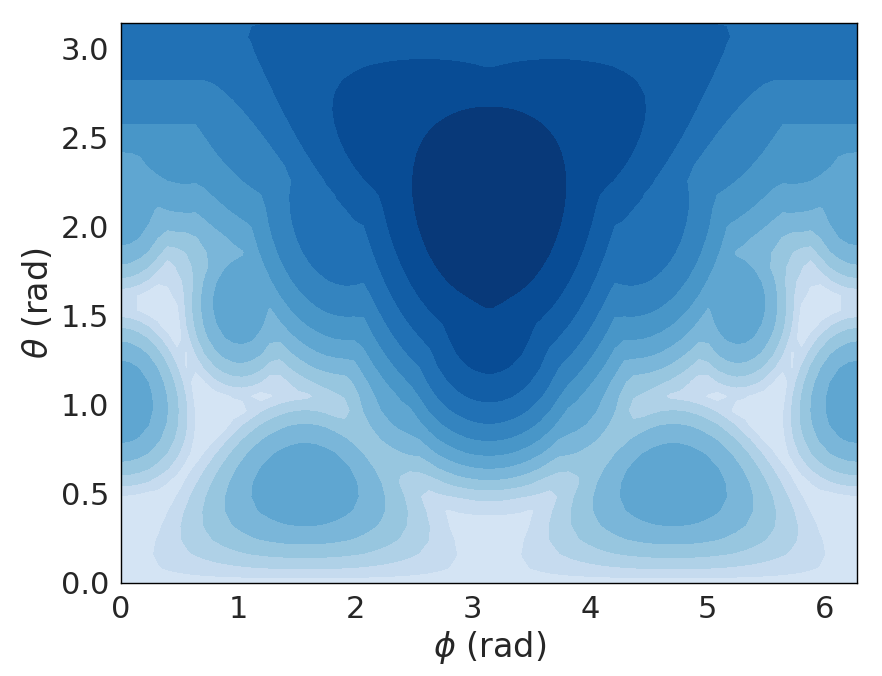
\includegraphics[height=.31\linewidth]{xzpsi-icos.png}}
        \subfigure[Rhombicuboctahedron]{\label{fig:hm-romb}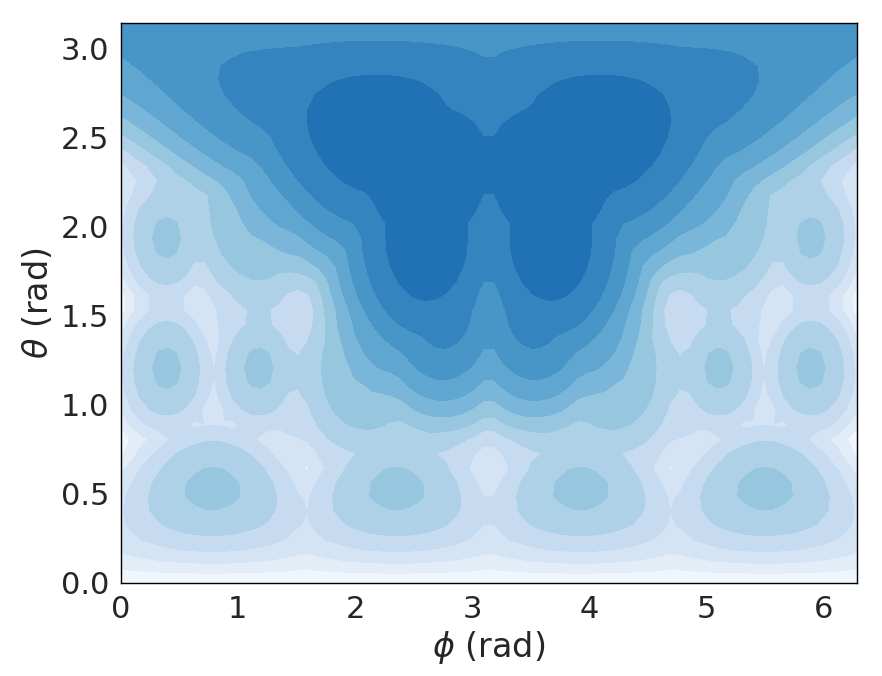
\includegraphics[height=.31\linewidth]{xzpsi-romb.png}}
        \subfigure{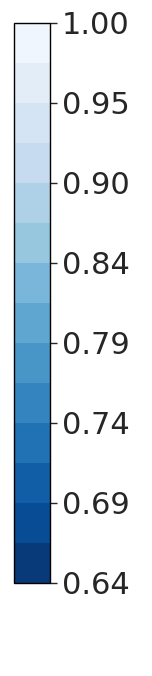
\includegraphics[height=.31\linewidth]{xzpsi-colorbar.png}}
        \caption{Application of program \eqref{eq:measurement-classicality-projective} to $\mathcal{S}(\theta, \phi) = \{ \rho_{\mathbf{x}}, \rho_{\mathbf{z}}, \rho_{\mathbf{r}(\theta, \phi)} \}$. Levels are the maximum visibility $\alpha$ such that preparation set $\alpha \mathcal{S}(\theta, \phi)$ has a classical model. \subref{fig:hm-icos} For the $Y = 6$ icosahedron measurements, $\eta \approx 0.79$, and program \eqref{eq:measurement-classicality-projective} can be directly applied. \subref{fig:hm-romb} A rhombicuboctahedron corresponds to $Y = 12$ projective measurements and $\eta \approx 0.86$. As the number of deterministic strategies scales exponentially, the computation of \subref{fig:hm-romb} is only possible by iteratively optimizing over subsets of deterministic strategies, as states in algorithm \ref{algo:iterative-strategy}.}
    \end{figure*}

	While our results are fully general, moving on to higher dimensions presents us with two considerable drawbacks. Similarly to the example discussed above, qudits will naturally lead to more extremal points in our classicality polytope, and ultimately to more computation time. Yet another considerable downside is that generating a large depolarized Bloch ball in larger dimensions will be costlier, while also the intuition brought by using polyhedra (with antipodal vertices) as a measurements polytope is lost. Howbeit, picking random $3$-qutrits preparations and $12$ random projective measurements (average $\eta \approx 0.26$), we found the mean computation time to be around $37$ minutes for each preparation set. Increasing the number of measurements and preparations is also possible by paying with more waiting until convergence is reached. In all cases, as each iteration returns a non-decreasing visibility $\alpha$, one will always obtain lower bounds even if convergence is not quickly attained. These observations lead us to argue that, with a clever selection of probe measurements, our method could still be useful for future applications even in larger dimensions.